%---------------
%╔═╗╔═╗╔╦╗╦ ╦╔═╗
%╚═╗║╣  ║ ║ ║╠═╝
%╚═╝╚═╝ ╩ ╚═╝╩  
%---------------

% language setup
\newcommand{\docLanguage}{ngerman}
%\newcommand{\docLanguage}{english}

% DOCUMENT SETUP
\documentclass[12pt, oneside, a4paper, \docLanguage]{report}
\usepackage[left=3cm, 
			right=2.5cm, 
			top=2.5cm, 
			bottom=2.5cm, 
			includehead, 
			includefoot]{geometry}

% line spacing
\usepackage{setspace}
\setstretch{1,25} % 15/12 --> 1.25

% encoding setup
% T1 font encoding for languages that use a latin alphabet
\usepackage[T1]{fontenc} 

% enhanced input encoding handling - utf8 for äÄüÜöÖß...
\usepackage[utf8]{inputenc}

%de­fines Adobe Times Ro­man as de­fault text font
\usepackage{mathptmx}
\usepackage{times} % needed for acronym package

%PDF linking package
\usepackage[hidelinks]{hyperref}

% Language Setup
\usepackage[\docLanguage]{babel}
% after babel - set chapter string
\AtBeginDocument{\renewcommand{\chaptername}{}}

% language specific bibliography style
\usepackage[numbers, square]{natbib}
%\setcitestyle{square,aysep={},yysep={;}}
\usepackage[fixlanguage]{babelbib}
\selectbiblanguage{\docLanguage}
% bliographystyle setup
% babel specific: babplain, babplai3, babalpha, babunsrt, bababbrv, bababbr3
\bibliographystyle{babunsrt}


% enumeration
\usepackage{enumitem}
% tabular extension tabularx
\usepackage{tabularx}

% math packages
\usepackage{amsmath}
\usepackage{nicefrac}
\usepackage{amsthm}
\usepackage{amsbsy}
\usepackage{amssymb}
\usepackage{amsfonts}
%\usepackage{MnSymbol}


%special characters
\usepackage{amssymb}
\usepackage{upgreek,textgreek}

% acronym package
\usepackage[printonlyused, footnote]{acronym}

% breakable text in \seqsplit{}
\usepackage{seqsplit}

% \textmu
\usepackage{textcomp}

% package provides a way to compile sections of a document using the same preamble as the main document
\usepackage{subfiles}

% driver-independent color extension - used by listings,tabularx
\usepackage[usenames,dvipsnames,table,xcdraw]{xcolor}

% -- SYNTAX HIGHLIGHTING --
\usepackage{listings}
%% bash command line Syntax Highlighting
\lstdefinestyle{BASH_CMD}{ 
  columns=fullflexible,            % copy pasteable listings
  language=bash,
  basicstyle=\small\sffamily,
  basicstyle   = \small \ttfamily,
  keywordstyle = [1]\small \ttfamily,
  keywordstyle = [2]\small \ttfamily,
  commentstyle = \small \ttfamily,
  numbers=none,
  captionpos=b, 
  breaklines=true,
  numberstyle=\tiny,
  numbersep=3pt,
  frame=tlrb,
  columns=fullflexible,
  backgroundcolor=\color{white!20},
  linewidth=\linewidth,
  literate=                        % replace in code
     {Ö}{{\"O}}1 
     {Ä}{{\"A}}1 
     {Ü}{{\"U}}1 
     {ß}{{\ss}}2 
     {ü}{{\"u}}1 
     {ä}{{\"a}}1 
     {ö}{{\"o}}1 
     {â}{{\^{a}}}1 
     {Â}{{\^{A}}}1 
     {ç}{{\c{c}}}1 
     {Ç}{{\c{C}}}1 
     {ğ}{{\u{g}}}1 
     {Ğ}{{\u{G}}}1 
     {ı}{{\i}}1 
     {İ}{{\.{I}}}1 
     {ş}{{\c{s}}}1 
     {Ş}{{\c{S}}}1 
}
 % adds style BASH_CMD
%% Matlab Syntax Highlighting
\colorlet{keyword}{blue!100!black!80}
\colorlet{STD}{Lavender}
\colorlet{comment}{green!90!black!90}
\definecolor{mygreen}{rgb}{0,0.6,0}
\definecolor{mygray}{rgb}{0.5,0.5,0.5}
\definecolor{mymauve}{rgb}{0.58,0,0.82}


\lstdefinestyle{BASH_SCRIPT}{ 
  language     = bash,
  basicstyle   = \footnotesize \ttfamily,
  keywordstyle = [1]\color{keyword}\bfseries,
  keywordstyle = [2]\color{STD}\bfseries,
  commentstyle = \color{mygreen}\itshape,
  backgroundcolor=\color{white},   % choose the background color; you must add \usepackage{color} 
  columns=fullflexible,            % copy pasteable listings
                                   % or \usepackage{xcolor}
  basicstyle=\footnotesize,        % the size of the fonts that are used for the code
  breakatwhitespace=false,         % sets if automatic breaks should only happen at whitespace
  breaklines=true,                 % sets automatic line breaking
  captionpos=b,                    % sets the caption-position to bottom
  extendedchars=true,              % lets you use non-ASCII characters; for 8-bits encodings only,
                                   % does not work with UTF-8
  frame=single,                    % adds a frame around the code
  keepspaces=true,                 % keeps spaces in text, useful for keeping indentation of code
                                   % (possibly needs columns=flexible)
  numbers=left,                    % where to put the line-numbers; possible values are 
                                   % (none, left, right)
  numbersep=5pt,                   % how far the line-numbers are from the code
  numberstyle=\tiny\color{mygray}, % the style that is used for the line-numbers
  rulecolor=\color{black},         % if not set, the frame-color may be changed on line-breaks
                                   % within not-black text (e.g. comments (green here))
  showspaces=false,                % show spaces everywhere adding particular underscores; it
  	                               % overrides 'showstringspaces'
  showstringspaces=false,          % underline spaces within strings only
  showtabs=false,                  % show tabs within strings adding particular underscores
  stepnumber=1,                    % the step between two line-numbers. If it's 1, each line 
                                   % will be numbered
  stringstyle=\color{mymauve},     % string literal style
  tabsize=2,                       % sets default tabsize to 2 spaces
  title=\lstname,                  % set title name
  literate=                        % replace in code
     {Ö}{{\"O}}1 
     {Ä}{{\"A}}1 
     {Ü}{{\"U}}1 
     {ß}{{\ss}}2 
     {ü}{{\"u}}1 
     {ä}{{\"a}}1 
     {ö}{{\"o}}1 
     {â}{{\^{a}}}1 
     {Â}{{\^{A}}}1 
     {ç}{{\c{c}}}1 
     {Ç}{{\c{C}}}1 
     {ğ}{{\u{g}}}1 
     {Ğ}{{\u{G}}}1 
     {ı}{{\i}}1 
     {İ}{{\.{I}}}1 
     {ş}{{\c{s}}}1 
     {Ş}{{\c{S}}}1 
} % adds style BASH_SCRIPT
% Matlab Syntax Highlighting
\colorlet{keyword}{blue!100!black!80}
\colorlet{STD}{red}
\colorlet{comment}{green!90!black!90}
\definecolor{mygreen}{rgb}{0,0.6,0}
\definecolor{mygray}{rgb}{0.5,0.5,0.5}
\definecolor{mymauve}{rgb}{0.58,0,0.82}


\lstdefinestyle{LATEX}{ 
  language     = [LaTeX]{TeX},
  basicstyle   = \footnotesize \ttfamily,
  keywordstyle = [1]\color{keyword}\bfseries,
  keywordstyle = [2]\color{comment}\bfseries,
  commentstyle = \color{mygray}\itshape,
  %backgroundcolor=\color{white},   % choose the background color; you must add \usepackage{color} 
                                   % or \usepackage{xcolor}
  basicstyle=\footnotesize,        		   % the size of the fonts that are used for the code
  breakatwhitespace=false,         % sets if automatic breaks should only happen at whitespace
  columns=fullflexible,            % copy pasteable listings
  breaklines=true,                 % sets automatic line breaking
  captionpos=c,                    % sets the caption-position to bottom
  extendedchars=true,              % lets you use non-ASCII characters; for 8-bits encodings only,
                                   % does not work with UTF-8
  frame=single,                    % adds a frame around the code
  keepspaces=true,                 % keeps spaces in text, useful for keeping indentation of code
                                   % (possibly needs columns=flexible)
  numbers=left,                    % where to put the line-numbers; possible values are 
                                   % (none, left, right)
  numbersep=4pt,                   % how far the line-numbers are from the code
  numberstyle=\tiny\color{mygray}, % the style that is used for the line-numbers
  rulecolor=\color{black},         % if not set, the frame-color may be changed on line-breaks
                                   % within not-black text (e.g. comments (green here))
  showspaces=false,                % show spaces everywhere adding particular underscores; it
  	                               % overrides 'showstringspaces'
  showstringspaces=false,          % underline spaces within strings only
  showtabs=false,                  % show tabs within strings adding particular underscores
  stepnumber=1,                    % the step between two line-numbers. If it's 1, each line 
                                   % will be numbered
  stringstyle=\color{mymauve},     % string literal style
  tabsize=2,                       % sets default tabsize to 2 spaces
  title=\lstname,                  % set title name
  literate=                        % replace in code
     {Ö}{{\"O}}1 
     {Ä}{{\"A}}1 
     {Ü}{{\"U}}1 
     {ß}{{\ss}}2 
     {ü}{{\"u}}1 
     {ä}{{\"a}}1 
     {ö}{{\"o}}1 
     {â}{{\^{a}}}1 
     {Â}{{\^{A}}}1 
     {ç}{{\c{c}}}1 
     {Ç}{{\c{C}}}1 
     {ğ}{{\u{g}}}1 
     {Ğ}{{\u{G}}}1 
     {ı}{{\i}}1 
     {İ}{{\.{I}}}1 
     {ş}{{\c{s}}}1 
     {Ş}{{\c{S}}}1 
} % adds style LATEX
%% Matlab Syntax Highlighting
\colorlet{keyword}{blue!100!black!80}
\colorlet{STD}{Lavender}
\colorlet{comment}{green!90!black!90}
\definecolor{mygreen}{rgb}{0,0.6,0}
\definecolor{mygray}{rgb}{0.5,0.5,0.5}
\definecolor{mymauve}{rgb}{0.58,0,0.82}


\lstdefinestyle{MATLAB}{ 
  language     = Matlab,
  basicstyle   = \footnotesize \ttfamily,
  keywordstyle = [1]\color{keyword}\bfseries,
  keywordstyle = [2]\color{STD}\bfseries,
  commentstyle = \color{mygreen}\itshape,
  backgroundcolor=\color{white},   % choose the background color; you must add \usepackage{color} 
                                   % or \usepackage{xcolor}
  basicstyle=\footnotesize,        % the size of the fonts that are used for the code
  breakatwhitespace=false,         % sets if automatic breaks should only happen at whitespace
  columns=fullflexible,            % copy pasteable listings
  breaklines=false,                % sets automatic line breaking
  captionpos=c,                    % sets the caption-position to bottom
  extendedchars=true,              % lets you use non-ASCII characters; for 8-bits encodings only,
                                   % does not work with UTF-8
  frame=single,                    % adds a frame around the code
  keepspaces=true,                 % keeps spaces in text, useful for keeping indentation of code
                                   % (possibly needs columns=flexible)
  numbers=left,                    % where to put the line-numbers; possible values are 
                                   % (none, left, right)
  numbersep=5pt,                   % how far the line-numbers are from the code
  numberstyle=\tiny\color{mygray}, % the style that is used for the line-numbers
  rulecolor=\color{black},         % if not set, the frame-color may be changed on line-breaks
                                   % within not-black text (e.g. comments (green here))
  showspaces=false,                % show spaces everywhere adding particular underscores; it
  	                               % overrides 'showstringspaces'
  showstringspaces=false,          % underline spaces within strings only
  showtabs=false,                  % show tabs within strings adding particular underscores
  stepnumber=1,                    % the step between two line-numbers. If it's 1, each line 
                                   % will be numbered
  stringstyle=\color{mymauve},     % string literal style
  tabsize=2,                       % sets default tabsize to 2 spaces
  title=\lstname,                  % set title name
  literate=                        % replace in code
     {Ö}{{\"O}}1 
     {Ä}{{\"A}}1 
     {Ü}{{\"U}}1 
     {ß}{{\ss}}2 
     {ü}{{\"u}}1 
     {ä}{{\"a}}1 
     {ö}{{\"o}}1 
     {â}{{\^{a}}}1 
     {Â}{{\^{A}}}1 
     {ç}{{\c{c}}}1 
     {Ç}{{\c{C}}}1 
     {ğ}{{\u{g}}}1 
     {Ğ}{{\u{G}}}1 
     {ı}{{\i}}1 
     {İ}{{\.{I}}}1 
     {ş}{{\c{s}}}1 
     {Ş}{{\c{S}}}1 
} % adds style MATLAB
% Matlab Syntax Highlighting
\colorlet{keyword}{blue!100!black!80}
\colorlet{STD}{Lavender}
\colorlet{comment}{green!90!black!90}
\definecolor{mygreen}{rgb}{0,0.6,0}
\definecolor{mygray}{rgb}{0.5,0.5,0.5}
\definecolor{mymauve}{rgb}{0.58,0,0.82}


\lstdefinestyle{PYTHON}{ 
  language     = Python,
  basicstyle   = \footnotesize \ttfamily,
  keywordstyle = [1]\color{keyword}\bfseries,
  keywordstyle = [2]\color{STD}\bfseries,
  commentstyle = \color{mygreen}\itshape,
  backgroundcolor=\color{white},   % choose the background color; you must add \usepackage{color} 
                                   % or \usepackage{xcolor}
  basicstyle=\footnotesize,        % the size of the fonts that are used for the code
  columns=fullflexible,            % copy pasteable listings
  breakatwhitespace=false,         % sets if automatic breaks should only happen at whitespace
  breaklines=false,                % sets automatic line breaking
  captionpos=c,                    % sets the caption-position to bottom
  extendedchars=true,              % lets you use non-ASCII characters; for 8-bits encodings only,
                                   % does not work with UTF-8
  frame=single,                    % adds a frame around the code
  keepspaces=true,                 % keeps spaces in text, useful for keeping indentation of code
                                   % (possibly needs columns=flexible)
  numbers=left,                    % where to put the line-numbers; possible values are 
                                   % (none, left, right)
  numbersep=5pt,                   % how far the line-numbers are from the code
  numberstyle=\tiny\color{mygray}, % the style that is used for the line-numbers
  rulecolor=\color{black},         % if not set, the frame-color may be changed on line-breaks
                                   % within not-black text (e.g. comments (green here))
  showspaces=false,                % show spaces everywhere adding particular underscores; it
  	                               % overrides 'showstringspaces'
  showstringspaces=false,          % underline spaces within strings only
  showtabs=false,                  % show tabs within strings adding particular underscores
  stepnumber=1,                    % the step between two line-numbers. If it's 1, each line 
                                   % will be numbered
  stringstyle=\color{mymauve},     % string literal style
  tabsize=2,                       % sets default tabsize to 2 spaces
  title=\lstname,                  % set title name
  literate=                        % replace in code
     {Ö}{{\"O}}1 
     {Ä}{{\"A}}1 
     {Ü}{{\"U}}1 
     {ß}{{\ss}}2 
     {ü}{{\"u}}1 
     {ä}{{\"a}}1 
     {ö}{{\"o}}1 
     {â}{{\^{a}}}1 
     {Â}{{\^{A}}}1 
     {ç}{{\c{c}}}1 
     {Ç}{{\c{C}}}1 
     {ğ}{{\u{g}}}1 
     {Ğ}{{\u{G}}}1 
     {ı}{{\i}}1 
     {İ}{{\.{I}}}1 
     {ş}{{\c{s}}}1 
     {Ş}{{\c{S}}}1 
} % adds style PYTHON
%% Matlab Syntax Highlighting
\colorlet{keyword}{blue!100!black!80}
\colorlet{STD}{Lavender}
\colorlet{comment}{green!90!black!90}
\definecolor{mygreen}{rgb}{0,0.6,0}
\definecolor{mygray}{rgb}{0.5,0.5,0.5}
\definecolor{mymauve}{rgb}{0.58,0,0.82}


\lstdefinestyle{CPP}{ 
  language     = C++,
  basicstyle   = \footnotesize \ttfamily,
  keywordstyle = [1]\color{keyword}\bfseries,
  keywordstyle = [2]\color{STD}\bfseries,
  commentstyle = \color{mygreen}\itshape,
  backgroundcolor=\color{white},   % choose the background color; you must add \usepackage{color} 
                                   % or \usepackage{xcolor}
  columns=fullflexible,            % copy pasteable listings
  basicstyle=\footnotesize,        % the size of the fonts that are used for the code
  breakatwhitespace=false,         % sets if automatic breaks should only happen at whitespace
  breaklines=false,                % sets automatic line breaking
  captionpos=c,                    % sets the caption-position to bottom
  extendedchars=true,              % lets you use non-ASCII characters; for 8-bits encodings only,
                                   % does not work with UTF-8
  frame=single,                    % adds a frame around the code
  keepspaces=true,                 % keeps spaces in text, useful for keeping indentation of code
                                   % (possibly needs columns=flexible)
  numbers=left,                    % where to put the line-numbers; possible values are 
                                   % (none, left, right)
  numbersep=5pt,                   % how far the line-numbers are from the code
  numberstyle=\tiny\color{mygray}, % the style that is used for the line-numbers
  rulecolor=\color{black},         % if not set, the frame-color may be changed on line-breaks
                                   % within not-black text (e.g. comments (green here))
  showspaces=false,                % show spaces everywhere adding particular underscores; it
  	                               % overrides 'showstringspaces'
  showstringspaces=false,          % underline spaces within strings only
  showtabs=false,                  % show tabs within strings adding particular underscores
  stepnumber=1,                    % the step between two line-numbers. If it's 1, each line 
                                   % will be numbered
  stringstyle=\color{mymauve},     % string literal style
  tabsize=2,                       % sets default tabsize to 2 spaces
  title=\lstname,                  % set title name
  literate=                        % replace in code
     {Ö}{{\"O}}1 
     {Ä}{{\"A}}1 
     {Ü}{{\"U}}1 
     {ß}{{\ss}}2 
     {ü}{{\"u}}1 
     {ä}{{\"a}}1 
     {ö}{{\"o}}1 
     {â}{{\^{a}}}1 
     {Â}{{\^{A}}}1 
     {ç}{{\c{c}}}1 
     {Ç}{{\c{C}}}1 
     {ğ}{{\u{g}}}1 
     {Ğ}{{\u{G}}}1 
     {ı}{{\i}}1 
     {İ}{{\.{I}}}1 
     {ş}{{\c{s}}}1 
     {Ş}{{\c{S}}}1 
} % adds style CPP
%% Matlab Syntax Highlighting
\colorlet{keyword}{blue!100!black!80}
\colorlet{STD}{Lavender}
\colorlet{comment}{green!90!black!90}
\definecolor{mygreen}{rgb}{0,0.6,0}
\definecolor{mygray}{rgb}{0.5,0.5,0.5}
\definecolor{mymauve}{rgb}{0.58,0,0.82}


\lstdefinestyle{C}{ 
  language     = C,
  basicstyle   = \footnotesize \ttfamily,
  keywordstyle = [1]\color{keyword}\bfseries,
  keywordstyle = [2]\color{STD}\bfseries,
  commentstyle = \color{mygreen}\itshape,
  backgroundcolor=\color{white},   % choose the background color; you must add \usepackage{color} 
  columns=fullflexible,            % copy pasteable listings
                                   % or \usepackage{xcolor}
  basicstyle=\footnotesize,        % the size of the fonts that are used for the code
  breakatwhitespace=false,         % sets if automatic breaks should only happen at whitespace
  breaklines=false,                % sets automatic line breaking
  captionpos=c,                    % sets the caption-position to bottom
  extendedchars=true,              % lets you use non-ASCII characters; for 8-bits encodings only,
                                   % does not work with UTF-8
  frame=single,                    % adds a frame around the code
  keepspaces=true,                 % keeps spaces in text, useful for keeping indentation of code
                                   % (possibly needs columns=flexible)
  numbers=left,                    % where to put the line-numbers; possible values are 
                                   % (none, left, right)
  numbersep=5pt,                   % how far the line-numbers are from the code
  numberstyle=\tiny\color{mygray}, % the style that is used for the line-numbers
  rulecolor=\color{black},         % if not set, the frame-color may be changed on line-breaks
                                   % within not-black text (e.g. comments (green here))
  showspaces=false,                % show spaces everywhere adding particular underscores; it
  	                               % overrides 'showstringspaces'
  showstringspaces=false,          % underline spaces within strings only
  showtabs=false,                  % show tabs within strings adding particular underscores
  stepnumber=1,                    % the step between two line-numbers. If it's 1, each line 
                                   % will be numbered
  stringstyle=\color{mymauve},     % string literal style
  tabsize=2,                       % sets default tabsize to 2 spaces
  title=\lstname,                  % set title name
  literate=                        % replace in code
     {Ö}{{\"O}}1 
     {Ä}{{\"A}}1 
     {Ü}{{\"U}}1 
     {ß}{{\ss}}2 
     {ü}{{\"u}}1 
     {ä}{{\"a}}1 
     {ö}{{\"o}}1 
     {â}{{\^{a}}}1 
     {Â}{{\^{A}}}1 
     {ç}{{\c{c}}}1 
     {Ç}{{\c{C}}}1 
     {ğ}{{\u{g}}}1 
     {Ğ}{{\u{G}}}1 
     {ı}{{\i}}1 
     {İ}{{\.{I}}}1 
     {ş}{{\c{s}}}1 
     {Ş}{{\c{S}}}1 
} % adds style C
%% JSON Syntax Highlighting
\colorlet{keyword}{blue!100!black!80}
\colorlet{STD}{Lavender}
\colorlet{comment}{green!90!black!90}
\definecolor{mygreen}{rgb}{0,0.6,0}
\definecolor{mygray}{rgb}{0.5,0.5,0.5}
\definecolor{mymauve}{rgb}{0.58,0,0.82}

\newcommand\JSONnumbervaluestyle{\color{blue}}
\newcommand\JSONstringvaluestyle{\color{red}}

\newif\ifcolonfoundonthisline

\makeatletter

\lstdefinelanguage{json}
{
  showstringspaces    = false,
  keywords            = {false,true},
  alsoletter          = 0123456789.,
  morestring          = [s]{"}{"},
  morestring          = [s]{'}{'},
  stringstyle         = \ifcolonfoundonthisline\JSONstringvaluestyle\fi,
  MoreSelectCharTable =%
    \lst@DefSaveDef{`:}\colon@json{\processColon@json},
  basicstyle          = \ttfamily,
  keywordstyle        = \ttfamily\bfseries,
}

% flip the switch if a colon is found in Pmode
\newcommand\processColon@json{
  \colon@json%
  \ifnum\lst@mode=\lst@Pmode%
    \global\colonfoundonthislinetrue%
  \fi
}

\lst@AddToHook{Output}{%
  \ifcolonfoundonthisline%
    \ifnum\lst@mode=\lst@Pmode%
      \def\lst@thestyle{\JSONnumbervaluestyle}%
    \fi
  \fi
  %override by keyword style if a keyword is detected!
  \lsthk@DetectKeywords% 
}

% reset the switch at the end of line
\lst@AddToHook{EOL}%
  {\global\colonfoundonthislinefalse}

\makeatother



\lstdefinestyle{JSON}{ 
  language     = json,
  basicstyle   = \footnotesize \ttfamily,
  keywordstyle = [1]\color{keyword}\bfseries,
  keywordstyle = [2]\color{STD}\bfseries,
  commentstyle = \color{mygreen}\itshape,
  backgroundcolor=\color{white},   % choose the background color; you must add \usepackage{color} 
                                   % or \usepackage{xcolor}
  basicstyle=\footnotesize,        % the size of the fonts that are used for the code
  columns=fullflexible,            % copy pasteable listings
  breakatwhitespace=false,         % sets if automatic breaks should only happen at whitespace
  breaklines=false,                % sets automatic line breaking
  captionpos=c,                    % sets the caption-position to bottom
  extendedchars=true,              % lets you use non-ASCII characters; for 8-bits encodings only,
                                   % does not work with UTF-8
  frame=single,                    % adds a frame around the code
  keepspaces=true,                 % keeps spaces in text, useful for keeping indentation of code
                                   % (possibly needs columns=flexible)
  numbers=left,                    % where to put the line-numbers; possible values are 
                                   % (none, left, right)
  numbersep=5pt,                   % how far the line-numbers are from the code
  numberstyle=\tiny\color{mygray}, % the style that is used for the line-numbers
  rulecolor=\color{black},         % if not set, the frame-color may be changed on line-breaks
                                   % within not-black text (e.g. comments (green here))
  showspaces=false,                % show spaces everywhere adding particular underscores; it
  	                               % overrides 'showstringspaces'
  showstringspaces=false,          % underline spaces within strings only
  showtabs=false,                  % show tabs within strings adding particular underscores
  stepnumber=1,                    % the step between two line-numbers. If it's 1, each line 
                                   % will be numbered
  stringstyle=\color{mymauve},     % string literal style
  tabsize=2,                       % sets default tabsize to 2 spaces
  title=\lstname,                  % set title name
  literate=                        % replace in code
     {Ö}{{\"O}}1 
     {Ä}{{\"A}}1 
     {Ü}{{\"U}}1 
     {ß}{{\ss}}2 
     {ü}{{\"u}}1 
     {ä}{{\"a}}1 
     {ö}{{\"o}}1 
     {â}{{\^{a}}}1 
     {Â}{{\^{A}}}1 
     {ç}{{\c{c}}}1 
     {Ç}{{\c{C}}}1 
     {ğ}{{\u{g}}}1 
     {Ğ}{{\u{G}}}1 
     {ı}{{\i}}1 
     {İ}{{\.{I}}}1 
     {ş}{{\c{s}}}1 
     {Ş}{{\c{S}}}1 
} % adds style JSON

% HEADLINE CFG
\usepackage{fancyhdr} % Headers and footers
\usepackage{lastpage}
\usepackage{ifthen}
\setlength{\headheight}{1.5cm}
%\pagestyle{fancy} % All pages have headers and footers
% override plain page style for \part, \chapter or 
% \maketitle, which implicit specifies plain page style
\fancypagestyle{plain} 
{
	\fancyhead[L]{}
	\fancyhead[C]{}
	\fancyhead[R]{}
	\fancyfoot[L]{}
	\fancyfoot[C]{\thepage}
	\fancyfoot[R]{}
}
% set list pagestyle
\fancypagestyle{preface} 
{
	\fancyhead[L]{}
	\fancyhead[C]{}
	\fancyhead[R]{}
	\fancyfoot[L]{}
	\fancyfoot[C]{\thepage}
	\fancyfoot[R]{}
}
% set default pagestyle
\fancypagestyle{default} 
{
	\fancyhead{} % Blank out the default header
	\fancyfoot{} % Blank out the default footer
	\fancyhead[L]{}
	\fancyhead[C]{}
	\fancyhead[R]{}
	\fancyfoot[L]{}
	\fancyfoot[C]{\thepage}
	\fancyfoot[R]{}
}
%\fancypagestyle{default} 
{
\fancyhead[L]{\ifthenelse{\isodd{\value{page}}}{\arabic{chapter} \rightmark}{}}
\fancyhead[R]{\thepage}
}

\renewcommand{\chaptermark}[1]{\markright{#1}{}}
\renewcommand{\sectionmark}[1]{\markright{#1}{}}
\renewcommand{\headrulewidth}{0pt}
\renewcommand{\footrulewidth}{0pt}

% PICTURE CFG 
\usepackage{verbatim}
\usepackage{graphicx}
\usepackage{epstopdf}
\usepackage{caption}
\usepackage[list=true,listformat=simple]{subcaption}
% floating prevention packages
\usepackage{float}    % used with [H] positioning parameter
\usepackage{placeins} % \FloatBarrier 
% tikz packages
\usepackage{tikz}
\usepackage{standalone}
\usepackage{pgfplots}


% include only specified tex files - uncommend here
\includeonly{preface/cover,
             preface/abstract,
             preface/tableofcontents,
             preface/listoffigures,
             preface/listoftables,
             preface/lstlistoflistings,
             appendix/bibliography}

\graphicspath{ {../Images/} }


%-------------------
%╔═╗╔╦╗╦═╗╦╔╗╔╔═╗╔═╗
%╚═╗ ║ ╠╦╝║║║║║ ╦╚═╗
%╚═╝ ╩ ╩╚═╩╝╚╝╚═╝╚═╝
%-------------------
\newcommand{\strLecture}{Signale, Systeme und Sensoren}
\newcommand{\strDate}{\today}
\newcommand{\strAuthorA}{Tim Köhler}
\newcommand{\strAuthorB}{Roland Burke}
%\newcommand{\strAuthorC}{C. Author}
\newcommand{\strAuthorAEmail}{tim.koehler@htwg-konstanz.de}
\newcommand{\strAuthorBEmail}{roland.burke@htwg-konstanz.de}
%\newcommand{\strAuthorCEmail}{cauthor@htwg-konstanz.de}
% Versuchsbeschreibung 
\newcommand{\strTopic}{Kalibrierung von Digitalkameras}
\newcommand{\strAbstract}{In diesem Versuch werden die Eigenschaften von digitalen Kameras untersucht. Wir führen dazu eine Kalibrierung des Kamerasensors durch, wie sie etwa bei industriellen Inspektionsanlagen, bei der Fernerkundung durch Satelliten oder in der Astronomie gemacht wird.
Dieser Prozess ist in 4 Teile aufgeteilt:\newline
\begin{enumerate}
\item \textbf{Aufnahme und Analyse eines Grauwertkeiles}\newline
In dieser Teilaufgabe wird ein Bild eines Grauwertkeils mit Hilfe von Python aufgenommen und der Mittelwert sowie die Standartabweichung der einzelnen Stufen berechnet.
\item \textbf{Aufnahme eines Dunkelbilder}\newline
Hier werden 10 Bilder mit abgedeckter Kamera gemacht(Dunkelbilder) und anschließend der Mittelwert eines jeden Pixels der 10 Bilder zu einen neuen Durchschnittsbild berechnet.
\item \textbf{Aufnahme eines Weißbildes}\newline
Gleich wie bei bei Aufgabe 2.
\item \textbf{Pixelfehler}\newline
Die letzte Aufgabe beinhaltet die Reparatur von \textit{dead pixels}, \textit{stuck pixels} und \textit{hot pixels} in	den Ursprungsbildern
\end{enumerate}
}
% hyperref customization
\hypersetup{
	pdftitle     = {\strTopic}, % title
	pdfsubject   = {\strLecture}, % subject of the document
	pdfauthor    = {\strAuthorA, \strAuthorB}, % author
	pdfkeywords  = {}, % list of keywords
	pdfcreator   = {}, % creator of the document
	pdfproducer  = {}, % producer of the document
	colorlinks   = false, % false: boxed links; true: colored links
	linkcolor    = red, % color of internal links (change box color with linkbordercolor)
    citecolor    = green, % color of links to bibliography
    filecolor    = magenta, % color of file links
    urlcolor     = cyan, % color of external links
	%bookmarks    = true, % show bookmarks bar?
	unicode	     = true, % non-Latin characters in Acrobat’s bookmarks
	pdftoolbar   = true, % show Acrobat’s toolbar?
	pdfmenubar   = true, % show Acrobat’s menu?
    pdffitwindow = false, % window fit to page when opened
	pdfnewwindow = true % links in new PDF window
}

%-----------------------------------------
% ╔╗ ╔═╗╔═╗╦╔╗╔  ╔╦╗╔═╗╔═╗╦ ╦╔╦╗╔═╗╔╗╔╔╦╗ 
% ╠╩╗║╣ ║ ╦║║║║   ║║║ ║║  ║ ║║║║║╣ ║║║ ║  
% ╚═╝╚═╝╚═╝╩╝╚╝  ═╩╝╚═╝╚═╝╚═╝╩ ╩╚═╝╝╚╝ ╩  
%-----------------------------------------

\begin{document}
\pagenumbering{Roman} 

\setcounter{section}{0}

\begin{titlepage}

\vspace*{-3.5cm}

\begin{flushleft}
\hspace*{-1cm} 
\includegraphics[width=15.7cm]{preface/htwg-logo}
\end{flushleft}

\vspace{1cm}

\begin{center}
	\large{
		\textbf{\strLecture} \\[2cm]
	}
	\Huge{
		\textbf{\strTopic} \\[2cm]
	}
	\Large{
		\textbf{\strAuthorA, \strAuthorB}} \\[3cm]
		%\textbf{\strAuthorA, \strAuthorB, \strAuthorC}} \\[3cm]
	\large{
		\textbf{} \\[2.3cm]
	}
	
	\large{
		\textbf{Konstanz, \strDate}
	}
\end{center}

\end{titlepage}
\thispagestyle{empty}




\begin{center}
{\Large \textbf{Zusammenfassung (Abstract)}}
\end{center}

\bigskip

\begin{center}
	\begin{tabular}{p{2.8cm}p{5cm}p{5cm}}
		Thema: & \multicolumn{2}{p{10cm}}{\raggedright\strTopic} \\
		 & & \\
		Autoren: & \strAuthorA & \href{mailto:\strAuthorAEmail}{\strAuthorAEmail} \\
		 & \strAuthorB & \href{mailto:\strAuthorBEmail}{\strAuthorBEmail} \\
%		 & \strAuthorC & \href{mailto:\strAuthorCEmail}{\strAuthorCEmail} \\
		 & & \\
		Betreuer: & Prof. Dr. Matthias O. Franz & \href{mailto:mfranz@htwg-konstanz.de}{mfranz@htwg-konstanz.de} \\
		 &  Jürgen Keppler & \href{mailto:juergen.keppler@htwg-konstanz.de}{juergen.keppler@htwg-konstanz.de} \\
		 &  Mert Zeybek & \href{mailto:me431zey@htwg-konstanz.de}{me431zey@htwg-konstanz.de} \\
	\end{tabular}
\end{center}

\bigskip

\noindent
\strAbstract

\thispagestyle{preface}



\clearpage

%
% TABLE OF CONTENTS
%
\pagestyle{preface}
%
% TABLE OF CONTENTS
%
\tableofcontents
\newpage


%
% Abbildungsverzeichnis
%
%
% Abbildungsverzeichnis
%
\phantomsection
\addcontentsline{toc}{chapter}{Abbildungsverzeichnis}
\listoffigures
\thispagestyle{preface}
\newpage
\clearpage

%
% Tabellenverzeichnis
%
%%
% Tabellenverzeichnis
%
\phantomsection
\addcontentsline{toc}{chapter}{Tabellenverzeichnis}
\listoftables
\thispagestyle{preface}
\newpage
\clearpage

%
% Listingverzeichnis
%
%
% Listingverzeichnis
%
\phantomsection
\renewcommand\lstlistingname{Listing}
\renewcommand\lstlistlistingname{Listingverzeichnis}
\lstlistoflistings
\addcontentsline{toc}{chapter}{Listingverzeichnis}
\thispagestyle{preface}
\newpage
\clearpage


%--------------------------
% ╔═╗╦ ╦╔═╗╔═╗╔╦╗╔═╗╦═╗╔═╗ 
% ║  ╠═╣╠═╣╠═╝ ║ ║╣ ╠╦╝╚═╗ 
% ╚═╝╩ ╩╩ ╩╩   ╩ ╚═╝╩╚═╚═╝ 
%--------------------------

\pagenumbering{arabic} 
\setcounter{page}{1} 
\pagestyle{default}
%
% CHAPTER Einleitung
%
\chapter{Einleitung}
\label{chap:EINL}
\begin{normalsize}
Digitale Kameras werden heutzutage überall eingesetzt. Jeder der heute ein Smartphone bestizt, hat auch eine oder sogar mehrere digital Kameras dabei. Außerdem werden solche Kameras bei Satelliten, industriellen Inspektionsanlagen oder zum Beispiel in autonom fahrenden Autos verwendet. Diese funktionieren aber nicht immer einwandfrei und deshalb wollen wir in diesem Versuch eine Digitalkamera kalibrieren und auf Fehler, wie beispielsweise nicht funktionierende Pixel, untersuchen. In unserem Fall untersuchen wir eine Logitech Webcam am Arbeitsplatz im Labor.
\end{normalsize}


%
% CHAPTER Versuch 1
%
\chapter{Versuch 1}
\label{chap:VERSUCH_1}

\section{Fragestellung, Messprinzip, Aufbau, Messmittel}
\label{chap:VERSUCH_1_FRAGESTELLUNG}
\begin{normalsize}
\textbf{Fragestellung:}\newline
In diesem Versuch überprüfen wir, wie gut die Webcam am Arbeitsplatz einen stufenförmigen
Grauwertverlauf aufnehmen kann.\newline
\textbf{Aufbau:}\newline
\end{normalsize}
\begin{figure}[H]
\centering
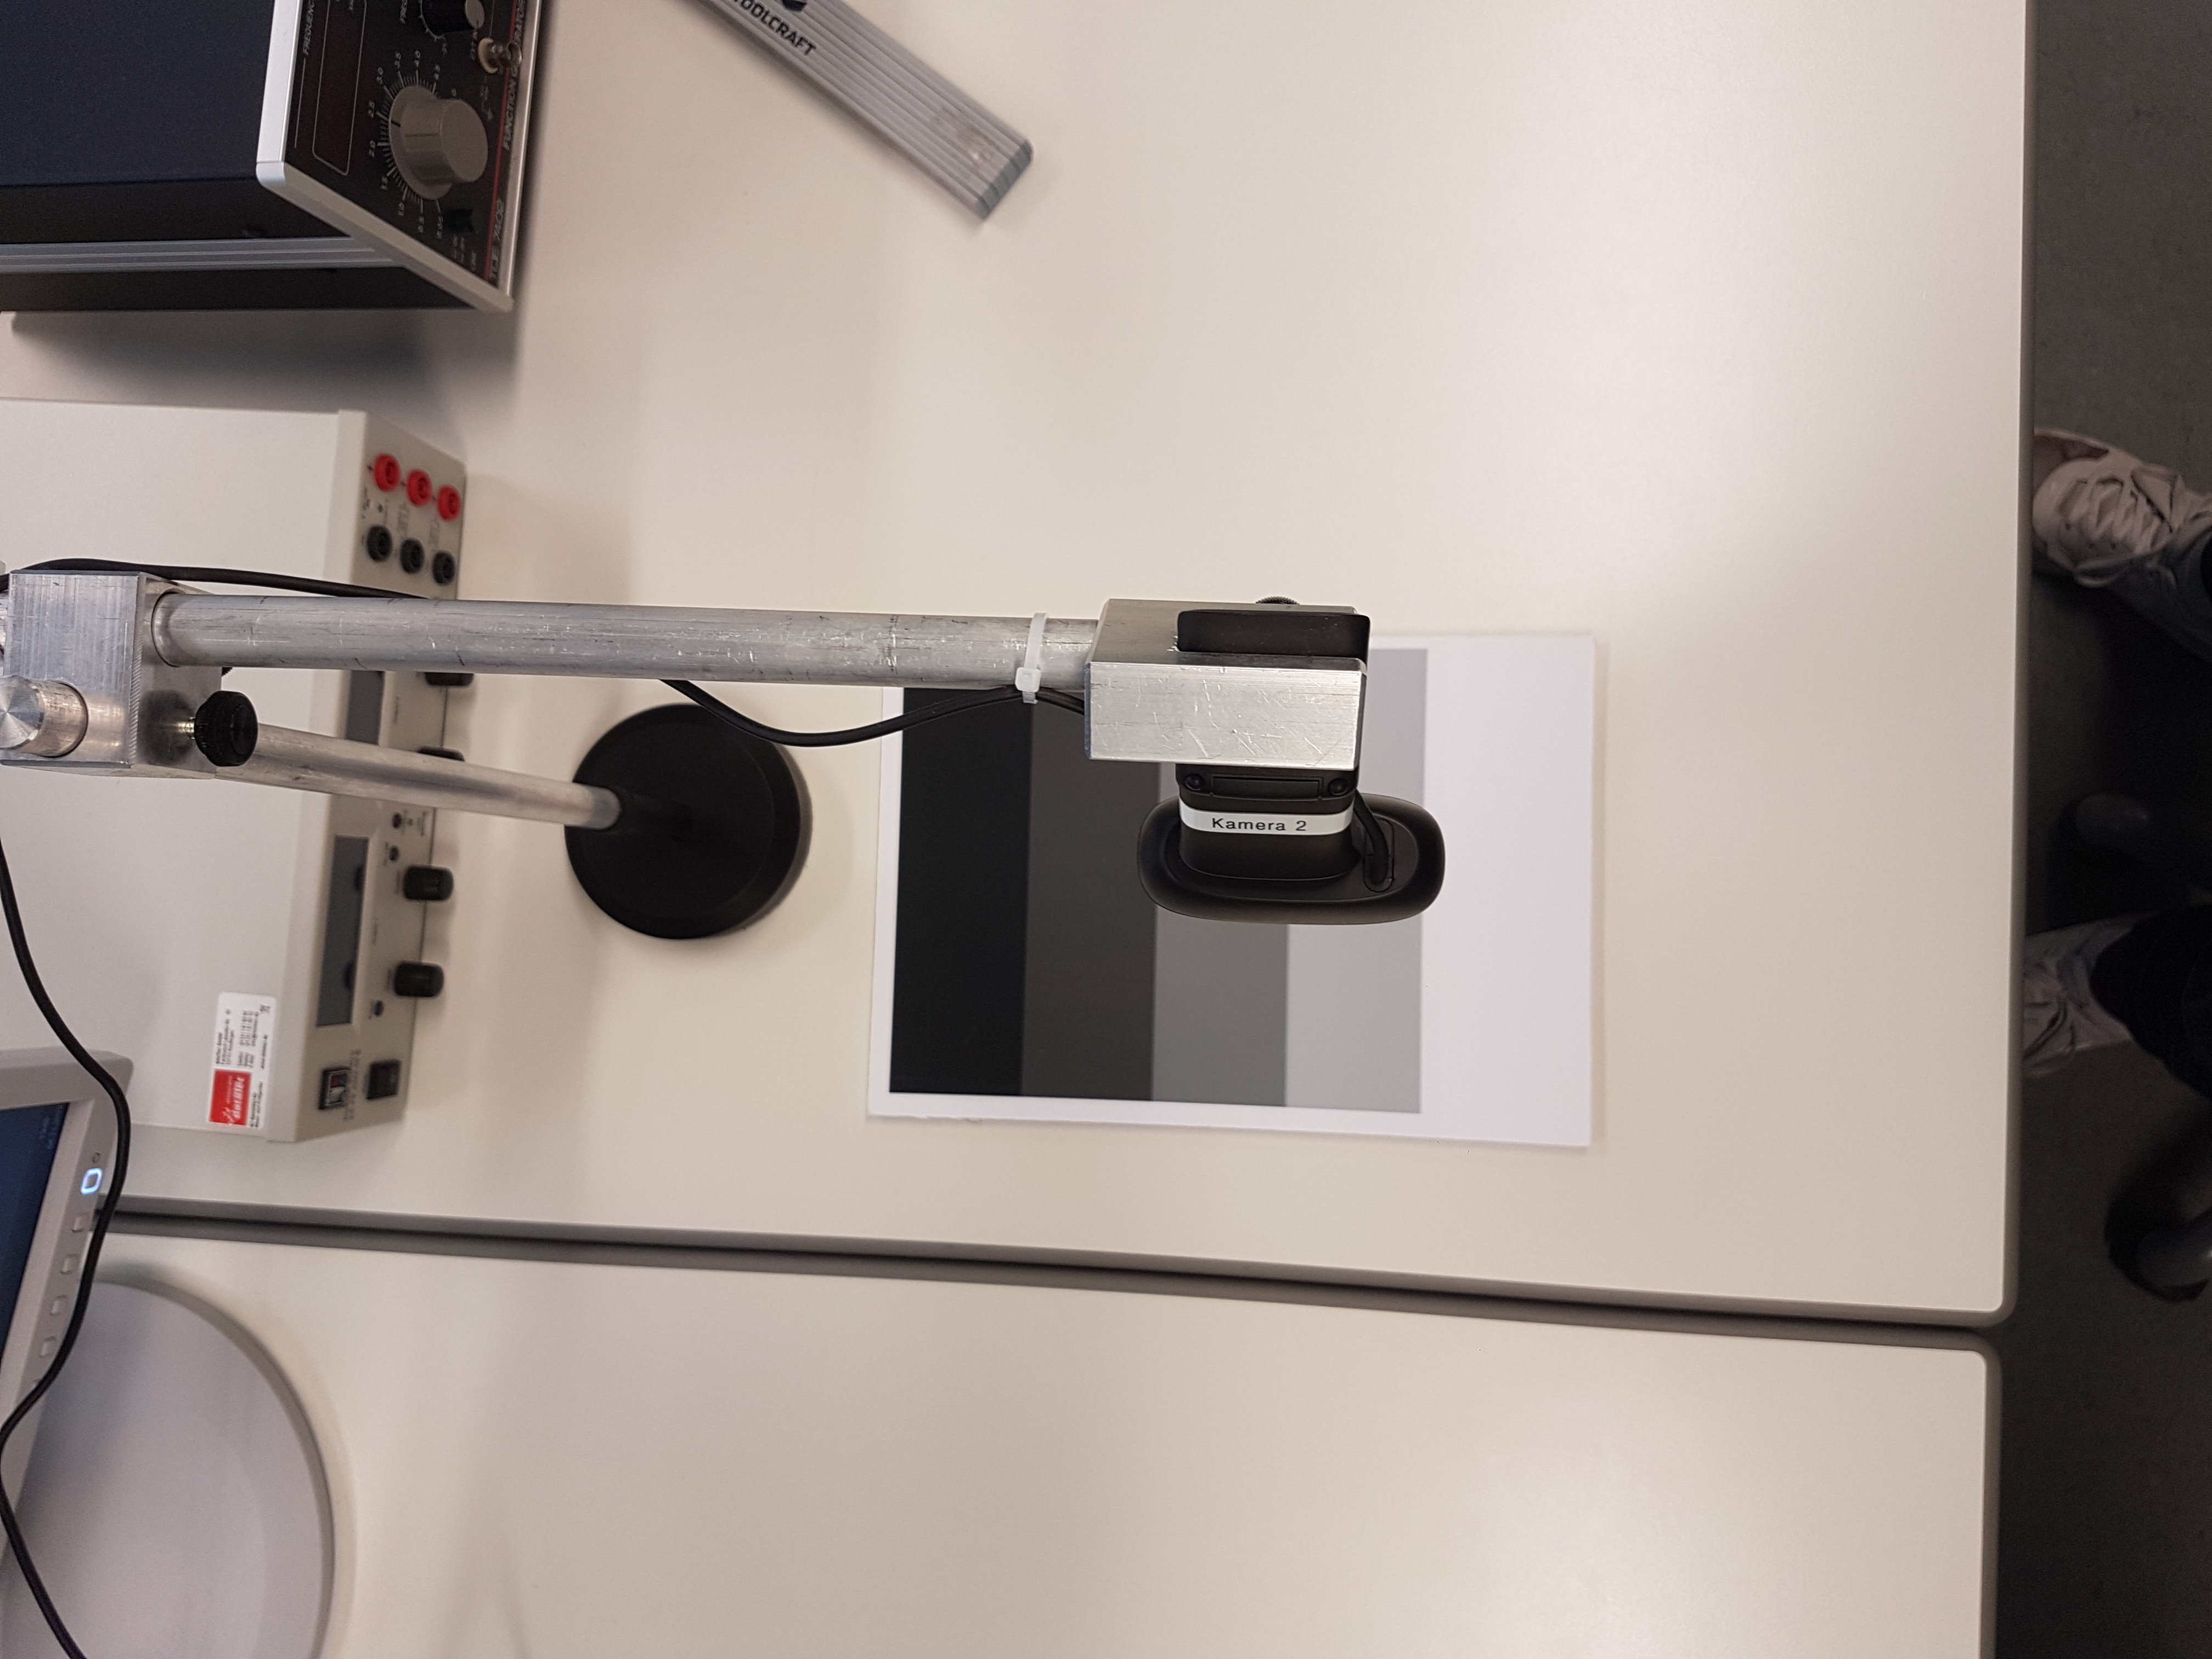
\includegraphics[scale=0.08]{Versuchsaufbau2.jpg}
\caption{Versuchsaufbau}
\end{figure}
\pagebreak
\textbf{Messmittel:}
\begin{itemize}
\item Logitech Webcam
\item Grauwertkeil
\item opencv (Python)
\end{itemize}

\section{Messwerte}
\label{chap:VERSUCH_1_MESSWERTE}
\begin{normalsize}
Das Bild des Grauwertkeils sieht folgendermaßen aus:
\end{normalsize}
\begin{figure}[H]
\centering
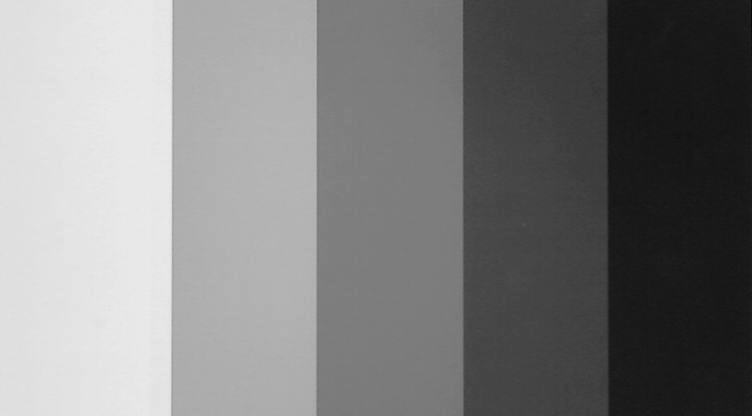
\includegraphics[scale=0.6]{../Greyscale.png}
\caption{Orginales Grauwertbild}
\end{figure}	
\pagebreak
\begin{flushleft}
Mit dem Histogram des Grauwertbildes kann ermittelt werden ob weiß oder schwarz in die Sättigung gehen.
\end{flushleft}
\begin{figure}[H]
\centering
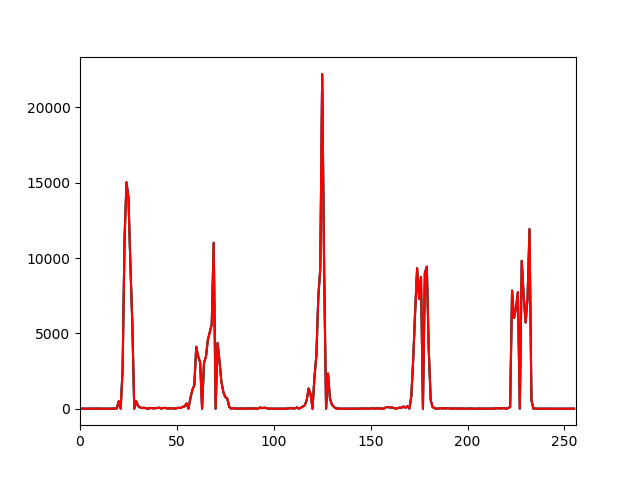
\includegraphics[scale=0.5]{./Histograms/HistGreyscale.png}
\caption{Historgram des Grauwertkeils}
\end{figure}

\section{Auswertung}
\label{chap:VERSUCH_1_AUSWERTUNG}
\begin{normalsize}
Mit \hyperref[chap:APPENDIX_SOURCECODE_V1]{\textit{diesem}} Python Script wird das Grauwertbild verarbeitet und in die folgenden Teilbilder zerschnitten:
\end{normalsize}
\begin{figure}[H]
\centering
\begin{subfigure}{.35\textwidth}
  \centering
  
\includegraphics[width=.35\linewidth]{../whiteSlice.png}
  \caption{Weiß}
  \label{fig:sub1}
\end{subfigure}
\begin{subfigure}{.35\textwidth}
  \centering
  
\includegraphics[width=.35\linewidth]{../whiteGreySlice.png}
  \caption{Weiß-Grau}
  \label{fig:sub2}
\end{subfigure}
\begin{subfigure}{.35\textwidth}
  \centering
  
\includegraphics[width=.35\linewidth]{../greySlice.png}
  \caption{Grau}
  \label{fig:sub3}
\end{subfigure}
\begin{subfigure}{.35\textwidth}
  \centering
  
\includegraphics[width=.35\linewidth]{../greyBlackSlice.png}
  \caption{Grau-Schwarz}
  \label{fig:sub4}
\end{subfigure}
\begin{subfigure}{.3\textwidth}
  \centering
  
\includegraphics[width=.35\linewidth]{../blackSlice.png}
  \caption{Schwarz}
  \label{fig:sub5}
\end{subfigure}
\caption{Teilbilder(Slices)}
\label{fig:Teilbilder}
\end{figure}
\pagebreak
\begin{flushleft}
Aus diesen Teilbildern berechnen wir dann den jeweiligen Mittelwert und die Standardabweichung:
\end{flushleft}

\begin{figure}[H]
\centering
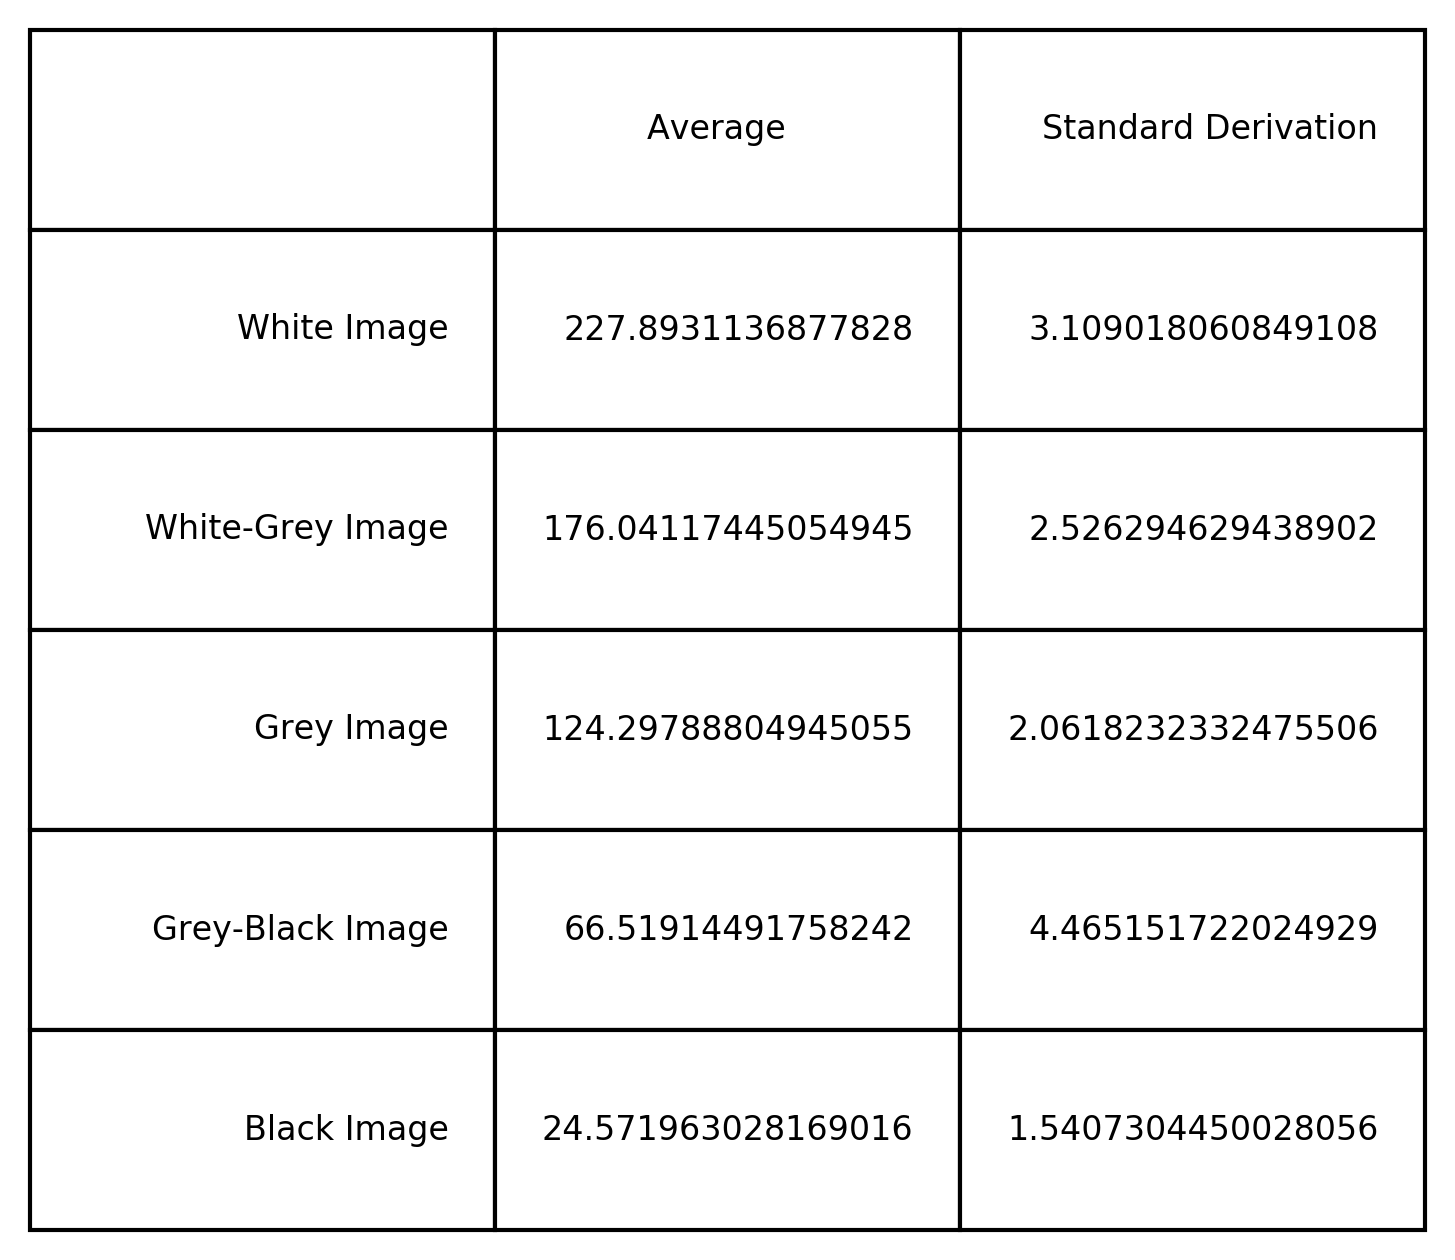
\includegraphics[scale=1.3]{../table.png}
\caption{Tabelle mit Mittelwert und Standartabweichung}
\end{figure}
\pagebreak

\section{Interpretation}
\label{chap:VERSUCH_1_INTERPRETATION}
Da das aufgenommene Muster vorher bekannt ist, kann
man anhand der Aufnahme die Wiedergabequalität messen. In unserem Fall sollte der
Grauwert innerhalb jeder Stufe konstant sein. Die reale Aufnahme wird aber aufgrund von
Bildfehlern und Sensorrauschen Abweichungen aufweisen.


%
% CHAPTER Versuch 2
%
\chapter{Versuch 2}
\label{chap:VERSUCH_2}

\section{Fragestellung, Messprinzip, Aufbau, Messmittel}
\label{chap:VERSUCH_2_FRAGESTELLUNG}

\begin{normalsize}
\textbf{Fragestellung:}\newline
Berechnung eines Mittelwert Dunkelbildes aus 10 Dunkelbildern\newline
\textbf{Messprinzip:}\newline
Nicht jeder Pixel einer Kamera liefert den Grauwert 0, wenn der Sensor abgedeckt ist. Das liegt
zum einen am thermischen Rauschen der Ausleseelektronik, zum anderen am sogenannten
Dunkelstrom, das aufgrund von Fertigungstoleranzen und von spontan durch Wärmezufuhr
entstehenden Ladungsträgerpaaren zu einem leicht unterschiedlichen Nullpunkt jedes Pixels
führt. Diesen pixelweisen Offset kann man durch Erstellung eines Dunkelbildes eliminieren,
den man von jeder Aufnahme subtrahiert.\newline
\textbf{Aufbau:}\newline
Hierzu wird einfach die Kamera zugehalten.\newline
\textbf{Messmittel:}\newline
Die in diesem Versuch verwendeten Mittel:
\begin{itemize}
\item Logitech Webcam
\item Python Script
\end{itemize}
\end{normalsize}

\section{Messwerte}
\label{chap:VERSUCH_2_MESSWERTE}
\begin{figure}[H]
\centering

\includegraphics[scale=0.5]{BlackImages/Black3.png}
\caption{Beispiel eines Dunkelbildes}
\end{figure}


\section{Auswertung}
\label{chap:VERSUCH_2_AUSWERTUNG}
Nach der Aufnahme der 10 Dunkelbilder wird mit hilfe \hyperref[chap:APPENDIX_SOURCECODE_V2]{\textit{dieses}} Python Prgramms der Mittelwert dieser Bilder bestimmt um das unten stehende Bild als Durchschnitt zu erzeugen:
\begin{figure}[H]
\centering

\includegraphics[scale=0.5]{../AverageBlackImage.png}
\caption{Durchschnittsbild der 10 Schwarzbilder}
\end{figure}


\section{Interpretation}
\label{chap:VERSUCH_2_INTERPRETATION}

\begin{normalsize}
Zunächst berechnen wird ein durchschnittliches Dunkelbild aus den 10 Dunkelbildern, damit die Korrektur genauer ist.
Mithilfe des Dunkelbildes kann man das thermische Ausleserauschen eliminieren, das heißt es bleibt nur noch der Offset bzw. der Dunkelstrom jedes Pixels übrig. Optimalerweise sollte das Dunkelbild komplett schwarz sein, so wie bei uns. Dies bedeutet schonmal, das es keine textit{stuck pixels} gibt, auf die wir später noch eingehen werden.\newline
\end{normalsize}

%
% CHAPTER Versuch 3
%
\chapter{Versuch 3}
\label{chap:VERSUCH_3}

\section{Fragestellung, Messprinzip, Aufbau, Messmittel}
\label{chap:VERSUCH_3_FRAGESTELLUNG}

\begin{normalsize}
\textbf{Fragestellung:}
\begin{itemize}
\item 10 Weißbilder aufnehmen
\item Ein Mittelwert Weißbildes aus 10 Weißbildern berrechnen, Dunkelbild abziehen und den Kontrast maximieren
\end{itemize}
\textbf{Messprinzip:}\newline
Obwohl die einzelnen Pixel einer Kamera eine hervorragende Linearität mit der Beleuchtungsstärke aufweisen, ist ihre Sensitivität aufgrund von Fertigungstoleranzen nicht völlig
gleich. Zusätzlich kommt noch die sogenannte Vignettierung hinzu, d.h. die Optik der Kamera
übeträgt die Helligkeit nicht gleichmäßig auf den Sensor. Typischerweise findet man eine
Abdunkelung des Bildes zu den Rändern hin. Zur Kompensation dieser Effekte nimmt man
ein sogenanntes Weißbild auf.\newline
\textbf{Aufbau:}\newline
Anstelle des Graukeils wird nun einfach ein weißes Papier vor die Linse gelegt.\newline
\textbf{Messmittel:}\newline
Die in diesem Versuch verwendeten Mittel:
\begin{itemize}
\item Logitech Webcam
\item Python Script
\item Weißes Blatt Papier
\end{itemize}
\end{normalsize}

\section{Messwerte}
\label{chap:VERSUCH_3_MESSWERTE}
\begin{figure}[H]
\centering
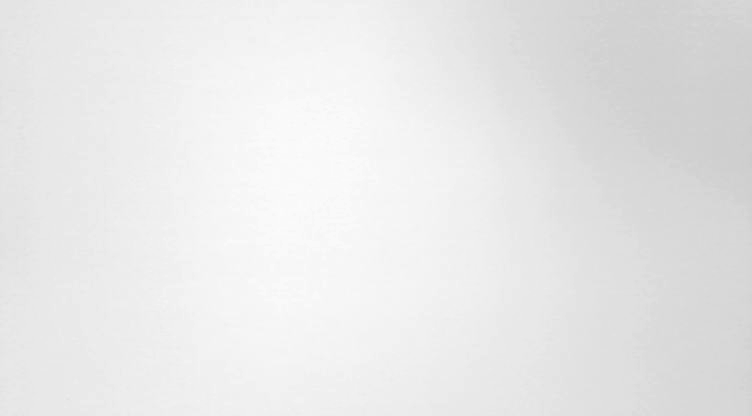
\includegraphics[scale=0.5]{WhiteImages/White3.png}
\caption{Beispiel eines Weißbildes}
\end{figure}

\section{Auswertung}
\label{chap:VERSUCH_3_AUSWERTUNG}
Nach der Aufnahme der 10 Weißbilder wird, genau wie bei den Schwarzbildern auch, aus dem Mittelwert dieser ein neues Bild erstellt. \hyperref[chap:APPENDIX_SOURCECODE_V3]{\textit{Dies}} ist der Code der zur Erstellung des folgenden Bildes verwendet wurde.
\begin{figure}[H]
\centering
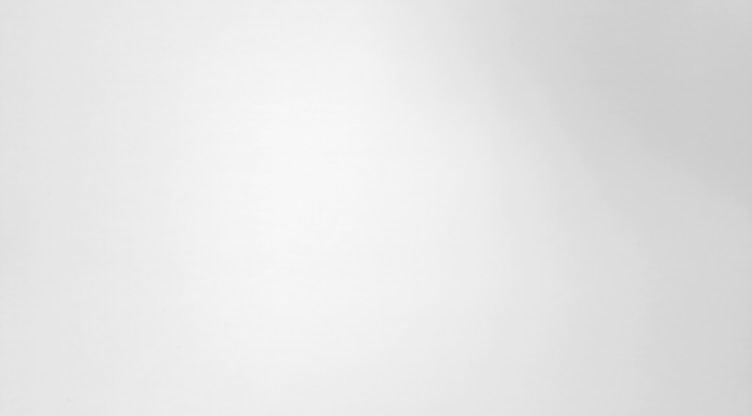
\includegraphics[scale=0.5]{../AverageWhiteImage.png}
\caption{Durchschnittsbild der 10 Weißbilder}
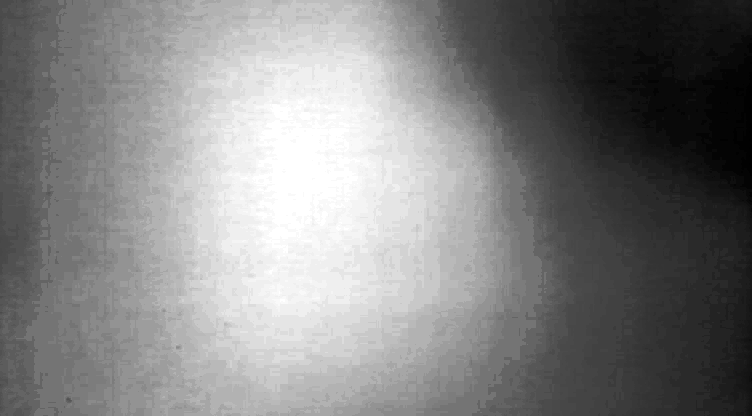
\includegraphics[scale=0.5]{../AverageWhiteImageMaxContrast.png}
\caption{Kontrastmaximiertes Weißbild}
\end{figure}
\pagebreak
\section{Interpretation}
\label{chap:VERSUCH_3_INTERPRETATION}

\begin{normalsize}
Durch Division durch das Weissbild kann man
die unterschiedlichen Sensitivitäten der einzelnen Pixel herausrechnen. Leider hängt das
Weißbild vom eingestellten Fokus des Kameraobjektives ab, d.h. im Prinzip braucht man für
jede Fokuseinstellung ein eigenes Weißbild. In unserem Fall bedeutet das, dass das Weißbild
in der gleichen Entfernung wie das zu korrigierende Bild aufgenommen werden muss.
Vom Gesichtspunkt der Kalibrierung her nehmen wir mit dem Weißbild einen zweiten Punkt
der Kennlinie jeden einzelnen Pixels auf. Zusammen mit dem Dunkelbild haben wir damit
die Kennlinie für alle Pixel gleichzeitig und eindeutig bestimmt: wir wissen an jeder Stelle des
Bildes die Steigung und den Nullpunkt und können durch Subtraktion des Dunkelbildes und
Division durch das Weißbild die tatsächliche Intensität des einfallenden Lichtes bestimmen.
Bei dem kontrastmaximierten Bild sind deutliche Kontraste zu sehen. Dies könnte an einer Reflektion einer Lampe liegen, die während der Aufnahme auf das Papier geleuchtet hat.\newline
\end{normalsize}

%
% CHAPTER Versuch 4
%
\chapter{Versuch 4}
\label{chap:VERSUCH_4}

\section{Fragestellung, Messprinzip, Aufbau, Messmittel}
\label{chap:VERSUCH_4_FRAGESTELLUNG}
\begin{normalsize}
\textbf{Fragestellung:}
\begin{itemize}
\item Überprüfung des Dunkelbilds auf \textit{stuck} und \textit{hot pixels} und das Weißbild auf \textit{dead pixels}
\item Korrektur des Grauwertbildes mit den Weiß- und Dunkelbildern aus den vorherigen Aufgaben
\end{itemize}
\textbf{Messprinzip:}\newline
Stuck und hot pixels entdeckt man am
einfachsten im Dunkelbild, bei dem diese Pixel als helle Punkte auffallen. Dead Pixels findet
man im Weißbild, wo sie als dunkle Punkte auffallen.\newline
\textbf{Aufbau:}\newline
Bei diesem Versuch gab es keinen Messaufbau.\newline
\textbf{Messmittel:}\newline
Die in diesem Versuch verwendeten Mittel:
\begin{itemize}
\item Dunkelbild
\item Weißbild
\item Python Script
\end{itemize}
\end{normalsize}

\section{Messwerte}
\label{chap:VERSUCH_4_MESSWERTE}
\begin{normalsize}
In diesem Versuch werden keine neuen Messungen getätigt. Es werden lediglich bereits erstellte Bilder aus den vorherigen Versuchen verwendet.
\end{normalsize}

\section{Auswertung}
\label{chap:VERSUCH_4_AUSWERTUNG}
\begin{normalsize}
Wir haben leider vergeblich nach \textit{stuck pixel} sowie \textit{hot pixel} in unseren Bildern gesucht.\newline
Der Quellcode für diese Aufgabe ist \hyperref[chap:APPENDIX_SOURCECODE_V4]{\textit{hier}} zu finden. 
\end{normalsize}
\begin{figure}[H]
\centering
\includegraphics[scale=0.6]{../GreyScaleCorrectedWithBlackWhiteImage.png}
\caption{Einfach korririerter Grauwertkeil}
\end{figure}
\begin{figure}[H]
\centering
\includegraphics[scale=0.6]{../2timesCorrectedGreyScale.png}
\caption{Doppelt korririerter Grauwertkeil}
\end{figure}
\begin{figure}[H]
\centering
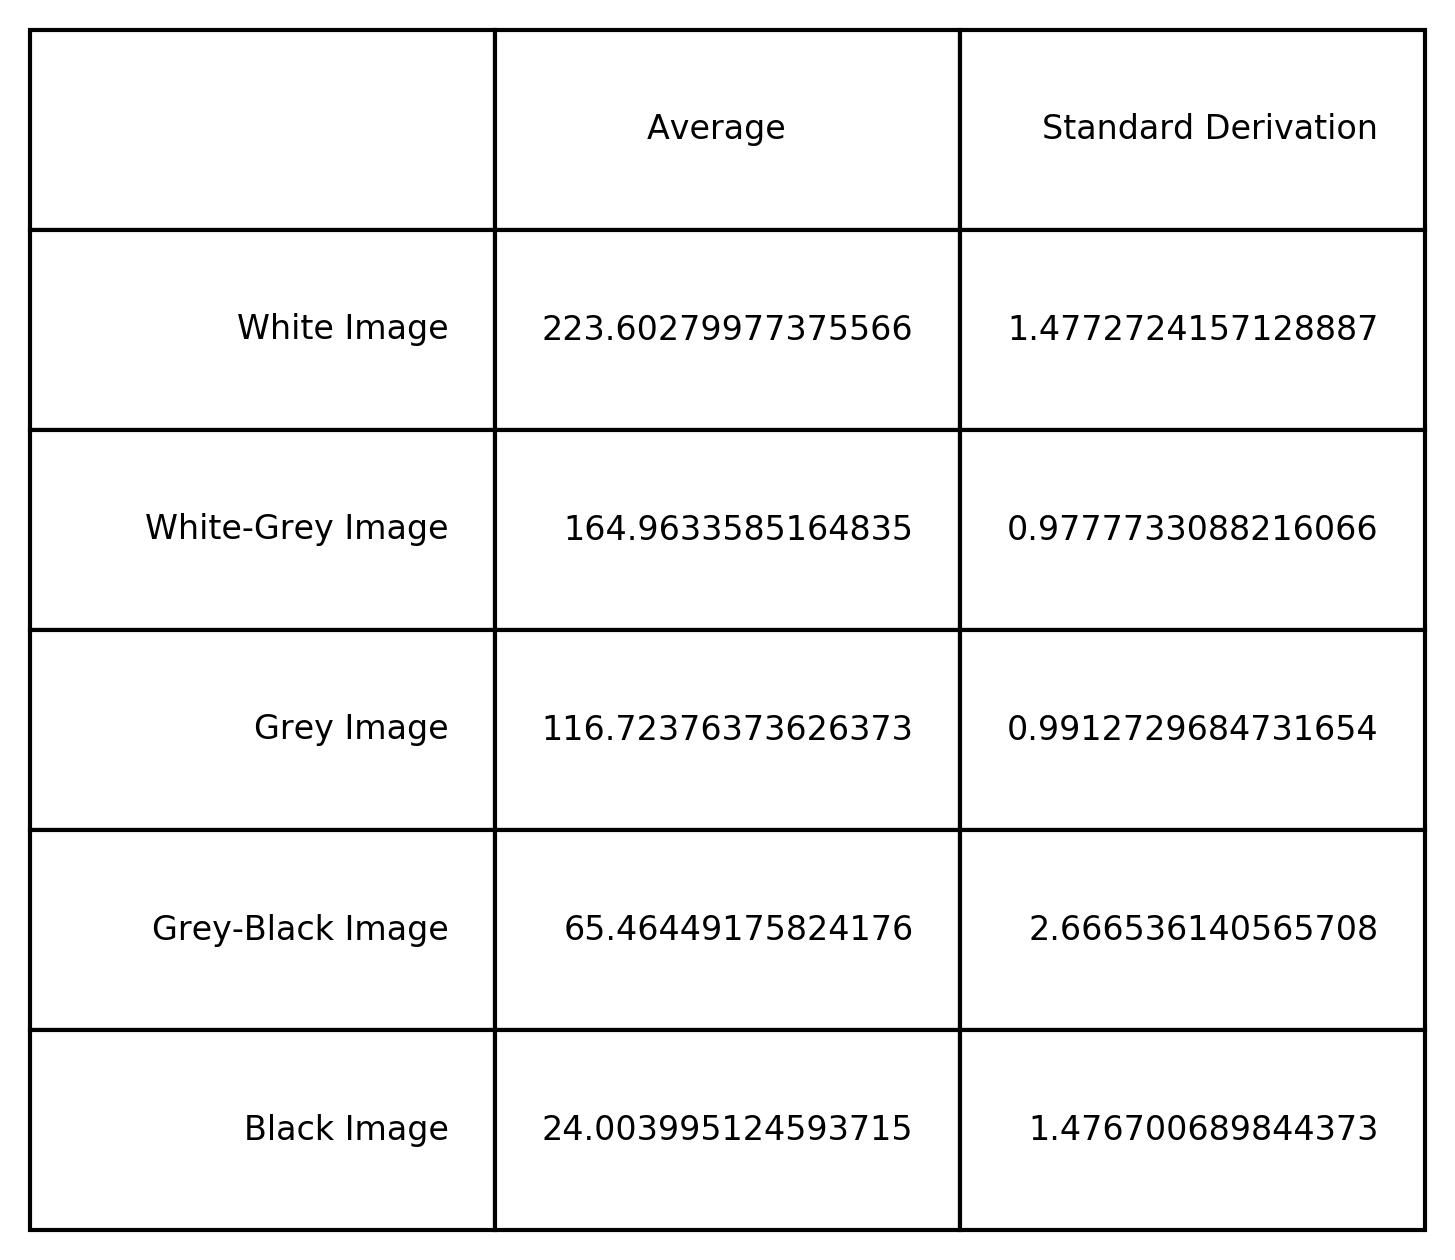
\includegraphics[scale=1]{../tableCorrected.png}
\caption{Tabelle des korrigierten Grawertkeils}
\end{figure}

\section{Interpretation}
\label{chap:VERSUCH_4_INTERPRETATION}
Je nach Qualität des Bildsensors entstehen beim Fertigungsprozess eine Anzahl von funktionsuntüchtigen Pixeln. Es gibt dead pixels, die immer auf ihrem niedrigsten Wert steckenbleiben,
stuck pixels, die immer auf ihrem Maximalwert bleiben, und sogenannte hot pixels, die bei längeren Belichtungszeiten in die Sättigung gehen.  Je nach Anwendung werden diese Pixelwerte im zu korrigierenden Bild durch Interpolation aus ihren Nachbarwerten ersetzt, so dass sie nicht mehr auffallen.\newline

%
% CHAPTER Anhang
%
\renewcommand\thesection{A.\arabic{section}}
\renewcommand\thesubsection{\thesection.\arabic{subsection}}

\chapter*{Anhang}
\label{chap:APPENDIX}
\addcontentsline{toc}{chapter}{Anhang}
%\setcounter{chapter}{0}
\addtocounter{chapter}{1}
\setcounter{section}{0}

\section{Quellcode}
\label{chap:APPENDIX_SOURCECODE}
\lstinputlisting[style=PYTHON, frame=single, captionpos=b, caption=Code zum aufnehmen der Bilder]{../CapureImage.py}
\pagebreak

\subsection{Quellcode Versuch 1}
\label{chap:APPENDIX_SOURCECODE_V1}
\lstinputlisting[style=PYTHON, frame=single, captionpos=b, caption=Code für Aufgabe 1]{../Task1.py}
\pagebreak

\subsection{Quellcode Versuch 2}
\label{chap:APPENDIX_SOURCECODE_V2}
\lstinputlisting[style=PYTHON, frame=single, captionpos=b, caption=Code für Aufgabe 2]{../Task2.py}

\pagebreak

\subsection{Quellcode Versuch 3}
\label{chap:APPENDIX_SOURCECODE_V3}
\lstinputlisting[style=PYTHON, frame=single, captionpos=b, caption=Code für Aufgabe 3]{../Task3.py}
\pagebreak

\subsection{Quellcode Versuch 4}
\label{chap:APPENDIX_SOURCECODE_V4}
\lstinputlisting[style=PYTHON, frame=single, captionpos=b, caption=Code für Aufgabe 4]{../ImproveImage.py}
\pagebreak

%\section{Messergebnisse}
%\label{chap:APPENDIX_MEASUREMENT_SOURCE}

%
% Literaturverzeichnis
%
%
% Literaturverzeichnis
%
\phantomsection
\addcontentsline{toc}{chapter}{Literaturverzeichnis}
\bibliography{references}
\newpage

\end{document}
%------------------------------------
% ╔═╗╔╗╔╔╦╗  ╔╦╗╔═╗╔═╗╦ ╦╔╦╗╔═╗╔╗╔╔╦╗
% ║╣ ║║║ ║║   ║║║ ║║  ║ ║║║║║╣ ║║║ ║ 
% ╚═╝╝╚╝═╩╝  ═╩╝╚═╝╚═╝╚═╝╩ ╩╚═╝╝╚╝ ╩ 
%------------------------------------